\section{Вступ}
Зі стрімким ростом об'єму інформації онлайн, класифікація тексту стала однією з ключових
технік для обробки та впорядкування даних. Галузі застосування є досить широкими:
починаючи від класифікації новин і закінчуючи персоналізованим пошуком відповідно до
потреб користувача. Оскільки побудова власного класифікатору є досить складним та
часозатратним процесом, доцільно розглянути приклади уже існуючих класифікаторів.
На сьогоднішній день існує величезна кількість алгоритмів, що використовуються для побудови прогностичних моделей. Прогностичні моделі – це математичні методи, що використовують статистику для передбачення майбутніх значень досліджуваної величини. Побудова таких моделей частіше за все здійснюється з метою передбачення поведінки величини у майбутньому, але загалом можуть бути використані для будь-якого типу події, незалежно від часу, коли вона відбулася.


\subsection{Прогностичне моделювання}
Прогностичне моделювання – використання статистичних методів для передбачення деякого цільового значення. Зазвичай, мається на увазі передбачення деякої величини в майбутньому, хоча узагальнено це не грає жодної ролі і може бути застосовано до будь-якого типу невідомої події, незалежно від того, коли вона відбулася.

В багатьох випадках задача зводиться до вибору найкращої моделі, що намагається здогадатися результат на основі набору вхідних даних, наприклад визначення того, чи є деякий лист електронної пошти спамом. Моделі можуть використовувати один чи декілька класифікаторів, щоб визначати приналежність даних до деякої множини. Сам термін прогностичної моделі широко перетинається з поняттями машинного навчання в наукових статтях та в контексті розробки програмного забезпечення. В промисловому середовищі даний термін швидше відноситься до поняття прогностичного аналізу.

Будь-яка регресійна модель може бути використана для прогностичних моделей. Загалом можна говорити про два класи прогностичних моделей: параметризовані та непараметризовані. Існує також суміжний третій клас, що поєднує властивості обох попередніх. Основна відмінність полягає в тому, що параметричні моделі роблять "визначені припущення, спираючись на один чи декілька параметрів, що характеризують закладений розподіл", в той час як непараметризовані не роблять жодних припущень на основі розподілу.

\subsubsection{Представлення та використання результатів прогностичних моделей}
Прогностичні моделі можуть бути використані безпосередньо, щоб отримати відповідь (результат) на основі вхідних характеристик (даних) або як компонент при здійсненні вибору на основі деяких правил.

В залежності від методології, що використовується для прогнозування, часто можна вивести деяку формулу-узагальнення (апроксимацію), що може бути використана в будь-якому додатку для роботи з таблицями. Це дає змогу працювати зі складними алгоритмами людям з досвідом роботи лише у офісних документах.

Номограми – графічні представлення прогностичних моделей. Перевагою такого представлення є можливість використання моделі без необхідної участі комп'ютера. Наприклад, деяка крива може бути використана на координатній площині для знаходження певної потрібної точки.

Дискретні оцінки – таблиця-представлення і найпростіший спосіб використання моделі. В рядках задається необхідне вхідне значення та вихідний параметр відповідно відображається в іншій колонці. Це може бути звичайна таблиця або деякий граф.

Окремим класом представлення є комп'ютерні додатки та веб-орієнтовані додатки, що дають аналогічне представлення у вигляді комп'ютерної програми з тюнінгом параметрів в режимі реального часу.

\subsubsection{Моделі росту}
Моделювання росту – це техніка, що показує зміну ймовірності в результаті певних дій. Наприклад, визначення того, чи клієнт залишиться покупцем певної компанії після випуску нового продукту. Модель дозволить вибрати оптимальну стратегію реклами серед покупців і економії грошей на існуючих клієнтах, що за даними прогностичної моделі залишаться покупцями незалежно від дій компанії.

Моделі, що будуються для визначення ймовірності прийняття клієнтом тих чи інших рішень. Використовуються для утримання клієнтів, маркетингу та продажів.

Модель може бути використана для оцінки ризиків виникнення інцидентів. Наприклад, дані про характеристики автомобіля та водійського стажу можуть слугувати показником ймовірності потрапляння в аварію.

Показники з медичних записів та історії хвороб пацієнтів можуть описувати моделі для визначення ризику виникнення захворювання чи необхідності повторного лікування.

Визначення ключових змінних, що впливають на ціну акцій, стоків, фьючерсів та курсу валют може бути використане для створення моделі, що побудує стратегію торгів та дасть змогу побудувати шаблони розвитку ринку. Щоправда, наразі невідомо жодної моделі, що на основі попередніх історичних даних могли б дати необхідні показники для успішної торгівлі на ринку.

Історичних даних не завжди достатньо для передбачення майбутніх даних. Використовуючи такі припущення ми вважаємо, що система має константні величини, від яких залежить система, що завжди хибни за умови участі людського фактору в будь-якій системі.

Не важливо, скільки факторів було враховано при зборі даних, завжди існує ймовірність, що нова, раніше не врахована змінна, викличе значний вплив на систему в майбутньому, що буде критично для попередньо розрахованих значень моделі.

Самопідтвердження алгоритму – якщо деякий алгоритм буде прийнято стандартом для вимірювань, особи, що мають інформацію про властивості алгоритму можуть використати його в особистих цілях та в цілях маніпуляції змінними, що не враховані в даному алгоритмі.


!HEREDOC Regression model

\begin{figure}[h!]
  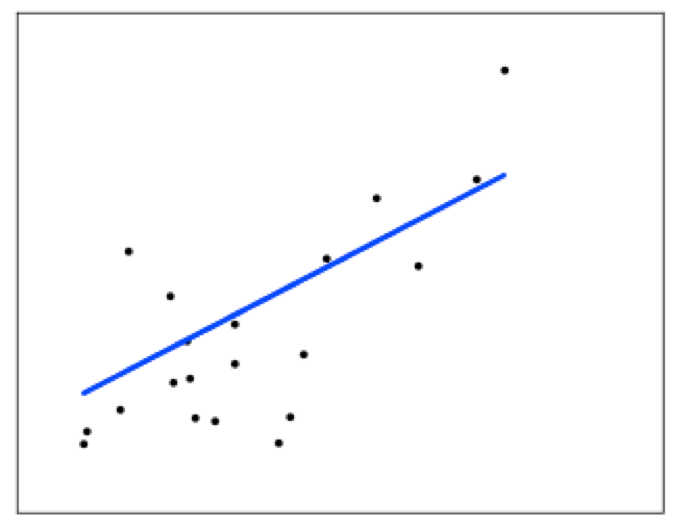
\includegraphics[width=\linewidth]{figures/linear_regression.png}
  \caption{Візуалізація лінійної регресії}
  \label{fig:linear_regression}
\end{figure}

